% \section{RoboDojo Benchmark}
% \label{sec:benchmark}

% Building on the system design described in Section~\ref{sec:method}, we construct the \textbf{\textcolor{Blue_1}{RoboDojo Benchmark}} for evaluating generalist robot manipulation policies. RoboDojo contains 42 simulation tasks and 18 real-world tasks. The simulation benchmark is designed for rapid feedback and model iteration, while providing comprehensive capability coverage through diverse task designs. Specifically, the simulation tasks are organized around five capability dimensions: Generalization, Memory, Precision, Long-Horizon, and Open-Ended Manipulation. These dimensions allow RoboDojo to analyze policy performance across distinct manipulation requirements, rather than only testing variations in objects, layouts, or language instructions. The real-world benchmark further exposes policies to challenging physical-world manipulation scenarios, where contact-rich dynamics, perception noise, actuation errors, and environmental variations can directly affect deployment performance. For simulation-based evaluation, RoboDojo supports heterogeneous multi-environment parallel evaluation on a single RTX 4090 GPU, allowing tasks with different configurations to be evaluated concurrently and improving evaluation speed for rapid simulation-based feedback. For real-world evaluation, RoboDojo provides a reproducible hardware setup and supports remote cloud-based evaluation, enabling participants from different locations to assess their policies under a shared physical evaluation protocol. Overall, RoboDojo provides a broad, challenging, and reproducible evaluation suite for diagnosing key limitations of current embodied manipulation policies.

% \begin{figure}[!t]
%     \centering
%     
\includegraphics[width=1.0\textwidth]{assets/Figure/tasks.pdf}
%     \caption{\textbf{\textcolor{Blue_1}{Tasks Overview of RoboDojo.}} 
%     RoboDojo contains 42 simulation tasks and 18 real-world tasks for evaluating generalist robot manipulation policies. The simulation tasks are organized around five complementary capability dimensions, including Generalization, Memory, Long-Horizon, Precision, and Open, providing diverse task structures for rapid feedback and model iteration. The real-world tasks are designed to expose policies to challenging physical-world manipulation scenarios under reproducible evaluation conditions. Together, these tasks cover a broad range of manipulation skills, spatial configurations, and bimanual coordination patterns, enabling comprehensive diagnosis of policy performance across simulation and the real world.}
%     \label{fig:all_tasks}
% \end{figure}

% \subsection{Simulation Benchmark}

% To support comprehensive and efficient simulation-based evaluation, we design 42 tasks on the ARX X5 bimanual platform, where the two arm bases are separated by 0.6 m. These tasks are organized around five capability dimensions: Generalization, Memory, Long-Horizon, Precision, and Open. The simulation benchmark is designed to provide rapid feedback for policy development, while covering diverse task structures and complementary manipulation requirements. In this way, RoboDojo evaluates policies beyond repeated variations of a narrow set of skills. Together with the heterogeneous parallel simulation described in Section~\ref{sec:parallelism}, this design improves evaluation speed and enables efficient model iteration across different capability dimensions. An overview of all simulation tasks is shown in Fig.~\ref{fig:all_tasks}, and detailed task definitions and visualizations are provided in Appendix~\ref{appendix:sim_benchmark_tasks_details} and on the \href{http://robodojo.com/doc}{project documentation for simulation task details}.


% \subsubsection{Task Design}

% \paragraph{Generalization.}
% A robot policy deployed outside a controlled laboratory should complete the same task across diverse environments, rather than only in a fixed scene with familiar visual conditions. This requires strong generalization to unseen backgrounds, lighting, clutter, and object appearances. The Generalization dimension contains 12 tasks that evaluate whether a policy can complete manipulation tasks under unseen condition variations, including changes in backgrounds, lighting, clutter configurations, and target objects. These tasks are designed to assess robustness to scene-level changes and the ability to identify task-relevant objects under diverse visual conditions. Compared with RoboTwin 2.0~\citep{chen2025robotwin}, RoboDojo introduces a larger range of scene randomization and more challenging tabletop clutter. While RoboTwin 2.0 includes at most 10 clutter objects on the table, RoboDojo randomizes up to 25 clutter objects, substantially increasing visual distraction and scene complexity. We believe that a truly generalizable policy should remain robust when deployed in unseen environments, rather than relying on a fixed visual context or a clean tabletop setup. To reduce overfitting to the default wooden-table scene and better preserve the generalization ability of policies, we additionally provide 100 DLC trajectories. These trajectories are not collected from the evaluation tasks themselves, but from simple pick-and-place behaviors under randomized backgrounds, lighting conditions, and clutter layouts. This design provides policies with broader visual exposure while avoiding direct leakage from the evaluation tasks.

% \paragraph{Memory.}
% Many manipulation tasks are partially observable, where the correct action depends on information observed earlier in the episode rather than only on the current frame. This requires the policy to retain task-relevant information over time, especially in non-Markovian manipulation scenarios. Inspired by RMBench~\citep{chen2026rmbench}, the Memory dimension contains 6 tasks that evaluate whether a policy can complete manipulation tasks when the necessary information is no longer directly visible at the time of action. These tasks are designed to assess the ability to maintain a sufficiently long observation history or use key-frame memory for decision making. For example, in \texttt{match\_and\_pick\_from\_conveyor}, the policy must remember the category of the first object that disappears on the conveyor and later pick the matching object among subsequently observed candidates. This requires the policy to act based on past visual evidence rather than only the current observation. Existing policies often rely on the current observation or a fixed-length observation window, which implicitly assumes that recent observations contain all necessary information for decision making. Such an assumption can fail in long-horizon and partially observable tasks, limiting the reliability and safety of policy execution in real-world manipulation.

% \paragraph{Long-Horizon.}
% Practical manipulation often requires completing a sequence of dependent steps before reaching the final goal. These tasks are challenging not only because they take longer to execute, but also because they require the policy to understand multi-step task structure, maintain progress over time, and execute actions consistently across an extended horizon. The Long-Horizon dimension contains 8 tasks that evaluate policy performance in extended multi-step manipulation scenarios. These tasks are designed to assess whether a policy can decompose a high-level instruction into a coherent action sequence and complete all required sub-steps without early termination or accumulated errors. For example, \texttt{classify\_objects} requires the robot to classify multiple objects into corresponding locations. Since the workspace is relatively large, the task may also involve handover behaviors between the two arms, resulting in long execution horizons and increased temporal complexity.

% \paragraph{Precision.}
% Fine-grained manipulation is essential for many everyday tasks, where small spatial errors or unstable motions can directly lead to failure. This requires the policy to accurately perceive target locations, predict smooth and robust trajectories, and execute precise contact-rich interactions. The Precision dimension contains 8 tasks that evaluate whether a policy can complete manipulation tasks with strict spatial and motion accuracy requirements. These tasks are designed to assess fine-grained visual grounding, trajectory smoothness, and local control stability. For example, in \texttt{insert\_tubes}, the policy must continuously insert tubes into narrow holes. This task becomes difficult when the predicted trajectory is not sufficiently smooth or spatially accurate, since even small errors can prevent successful insertion. Therefore, success in this dimension requires the policy to both clearly localize task-relevant targets from visual observations and generate stable actions for precise manipulation.

% \paragraph{Open.}
% Human instructions in open environments are not limited to a fixed task template, and may describe new goals using diverse language expressions. A generalist robot policy is therefore expected to understand diverse task specifications and transfer previously learned skills to new tasks. The Open dimension contains 8 tasks that evaluate whether a policy can solve unseen task specifications whose required skills have appeared in the training data under different contexts. These tasks are designed to assess open-semantic grounding, skill recombination, and language-conditioned transfer. For example, \texttt{general\_pickup} requires object grasping, which is a common skill repeatedly observed during training, but the specific grasping goal in this task is not directly included in the training tasks. This dimension evaluates whether policies can recombine learned manipulation skills and ground new language instructions to complete previously unseen tasks. In this way, it measures the policy's ability to generalize at the level of skill composition, task understanding, and semantic transfer.

\section{RoboDojo Benchmark}
\label{sec:benchmark}

Building on the system design in Section~\ref{sec:method}, we construct the \textbf{\textcolor{Blue_1}{RoboDojo Benchmark}} to evaluate generalist robot manipulation policies across simulation and the real world. RoboDojo consists of 42 simulation tasks and 18 real-world tasks. The simulation benchmark supports efficient model iteration and capability-oriented diagnosis across five dimensions: Generalization, Memory, Precision, Long-Horizon, and Open. These dimensions capture distinct manipulation requirements beyond variations in objects, layouts, or language instructions. The real-world benchmark complements simulation by evaluating policies under challenging physical deployment conditions with standardized and reproducible protocols. Together, RoboDojo provides a broad evaluation suite for systematically diagnosing the limitations of current embodied manipulation policies.

\begin{figure}[!t]
\centering

\includegraphics[width=1.0\textwidth]{assets/Figure/tasks.pdf}
\caption{\textbf{\textcolor{Blue_1}{Task Overview of RoboDojo.}}
RoboDojo includes 42 simulation tasks and 18 real-world tasks for evaluating generalist robot manipulation policies. The simulation tasks are organized into five capability dimensions: Generalization, Memory, Long-Horizon, Precision, and Open, enabling efficient capability-oriented diagnosis. The real-world tasks assess policy behavior under challenging and reproducible physical deployment conditions. Together, these tasks cover diverse manipulation skills, spatial configurations, and bimanual coordination patterns across simulation and the real world.}
\label{fig:all_tasks}
\end{figure}

\subsection{Simulation Benchmark}

We design 42 simulation tasks on the ARX X5 bimanual platform, with the two arm bases separated by 0.6,m. These tasks are organized into five capability dimensions: Generalization, Memory, Long-Horizon, Precision, and Open. The simulation benchmark is designed to provide rapid policy feedback and capability-oriented diagnosis beyond repeated variations of a narrow skill set. Together with the heterogeneous parallel simulation described in Section~\ref{sec:parallelism}, RoboDojo enables efficient model iteration across diverse task structures and manipulation requirements. An overview of all simulation tasks is shown in Fig.~\ref{fig:all_tasks}. Detailed task definitions and visualizations are provided in Appendix~\ref{appendix:sim_benchmark_tasks_details} and the \href{http://robodojo.com/doc}{project documentation}.

\subsubsection{Task Design}

\paragraph{Generalization.}
Robust deployment requires policies to complete the same task across diverse environments, rather than relying on fixed scenes or familiar visual contexts. The Generalization dimension includes 12 tasks that evaluate robustness to unseen variations in backgrounds, lighting, clutter, and target objects. Compared with RoboTwin 2.0~\citep{chen2025robotwin}, RoboDojo introduces stronger scene randomization and denser tabletop clutter. While RoboTwin 2.0 includes at most 10 clutter objects, RoboDojo randomizes up to 25 clutter objects, substantially increasing visual distraction and scene complexity. To further reduce overfitting to the default wooden-table scene, we provide 100 supplementary DLC trajectories for data-level augmentation. These trajectories are collected from simple pick-and-place behaviors under randomized backgrounds, lighting, and clutter layouts. Since they are independent of the evaluation tasks, they improve visual exposure without directly leaking task-specific solutions.

\paragraph{Memory.}
Many manipulation tasks are partially observable, where the correct action depends on information observed earlier rather than only the current frame. Inspired by RMBench~\citep{chen2026rmbench}, the Memory dimension includes 6 tasks that evaluate long-context observation modeling, key-frame memory, and non-Markovian decision making. These tasks cover both short-history settings, where a few key observations are sufficient for task completion, and longer interactive settings that require reasoning over multi-frame temporal sequences. For example, in \texttt{match\_and\_pick\_from\_conveyor}, the policy must remember the category of an object that disappears on the conveyor and later pick a matching object from subsequent candidates. In \texttt{imitate\_sorting\_sequence}, the policy observes another robot arm placing objects into a basket in a specific order, and must remember and reproduce the demonstrated ordering. These settings challenge policies that rely only on the current observation or a short fixed-length history.

\paragraph{Long-Horizon.}
Practical manipulation often requires executing a sequence of dependent steps before reaching the final goal. The Long-Horizon dimension includes 8 tasks that evaluate whether policies can infer task structure, maintain progress, and complete all required sub-steps without early termination or accumulated errors. For example, \texttt{classify\_objects} requires the robot to sort multiple objects into corresponding target locations. Due to the relatively large workspace, the task may also require handover behaviors between the two arms, resulting in longer execution horizons and increased temporal complexity.

\paragraph{Precision.}
Fine-grained manipulation requires accurate visual grounding, smooth motion prediction, and stable local control, since small spatial errors can directly lead to failure. The Precision dimension includes 8 tasks with strict spatial and motion accuracy requirements, focusing on fine-grained target localization, trajectory smoothness, and contact-rich control stability. For example, in \texttt{insert\_tubes}, the policy must continuously insert tubes into narrow holes. Even small localization or trajectory errors can prevent successful insertion, making this dimension particularly sensitive to action accuracy and motion stability.

\paragraph{Open.}
Generalist robot policies should understand diverse task specifications and transfer learned skills to new goals. The Open dimension includes 8 tasks that evaluate unseen task specifications whose required skills appear in the training data under different contexts. These tasks test open-semantic grounding, skill recombination, and language-conditioned transfer. For example, \texttt{general\_pickup} requires object grasping, a skill frequently observed during training, while the specific grasping goal is not directly included in the training tasks. This dimension examines whether policies can recombine learned manipulation skills and ground new language instructions to solve previously unseen tasks.


\subsubsection{Training Data Setting}

For simulation policy training, we provide 35 task directories with 3,500 trajectories, totaling 1,859,602 frames and 20.66 hours of bimanual manipulation data recorded at 25~Hz. These directories include 34 training tasks from the Generalization, Memory, Long-Horizon, and Precision dimensions, together with one auxiliary DLC data directory. Each training task contains 100 trajectories collected through either automated trajectory synthesis or VR-based teleoperation. The Open dimension is excluded from the training set, as it is designed to evaluate skill recombination and transfer to unseen task specifications rather than imitation of task-specific demonstrations.

For the Generalization dimension, demonstrations are collected under the standard setting without domain randomization. To reduce overfitting to a single visual configuration, we additionally include 100 auxiliary DLC trajectories for data-level augmentation. These trajectories are generated under complex domain randomization, including diverse backgrounds, lighting conditions, and clutter layouts. The auxiliary DLC data broadens visual exposure while remaining independent of the evaluation tasks, avoiding direct leakage of task-specific solutions. Detailed data modalities, collection procedures, and statistics are provided in Appendix~\ref{appendix:sim_training_data_statistics}.

\subsubsection{Evaluation Setting}

We evaluate policies on all 42 simulation tasks across five capability dimensions: Generalization, Memory, Long-Horizon, Precision, and Open. Each task is evaluated for 50 episodes, resulting in 2,100 episodes in total. We report both success rate and average score: success rate measures binary task completion, while average score captures partial task progress.

For the 12 Generalization tasks, the 50 episodes are split into 25 \textit{standard} episodes and 25 \textit{random} episodes. The \textit{standard} setting evaluates in-domain performance, whereas the \textit{random} setting introduces variations in backgrounds, clutter layouts, task-relevant objects, and lighting conditions to assess robustness under visual and scene-level distribution shifts. The overall performance is computed as the mean across the five capability dimensions, rather than across all tasks, preventing dimensions with more tasks from dominating the aggregate metric. Additional details on task horizons and episode settings are provided in Appendix~\ref{appendix:sim_evaluation_setting}.

\begin{figure}[t]
\centering
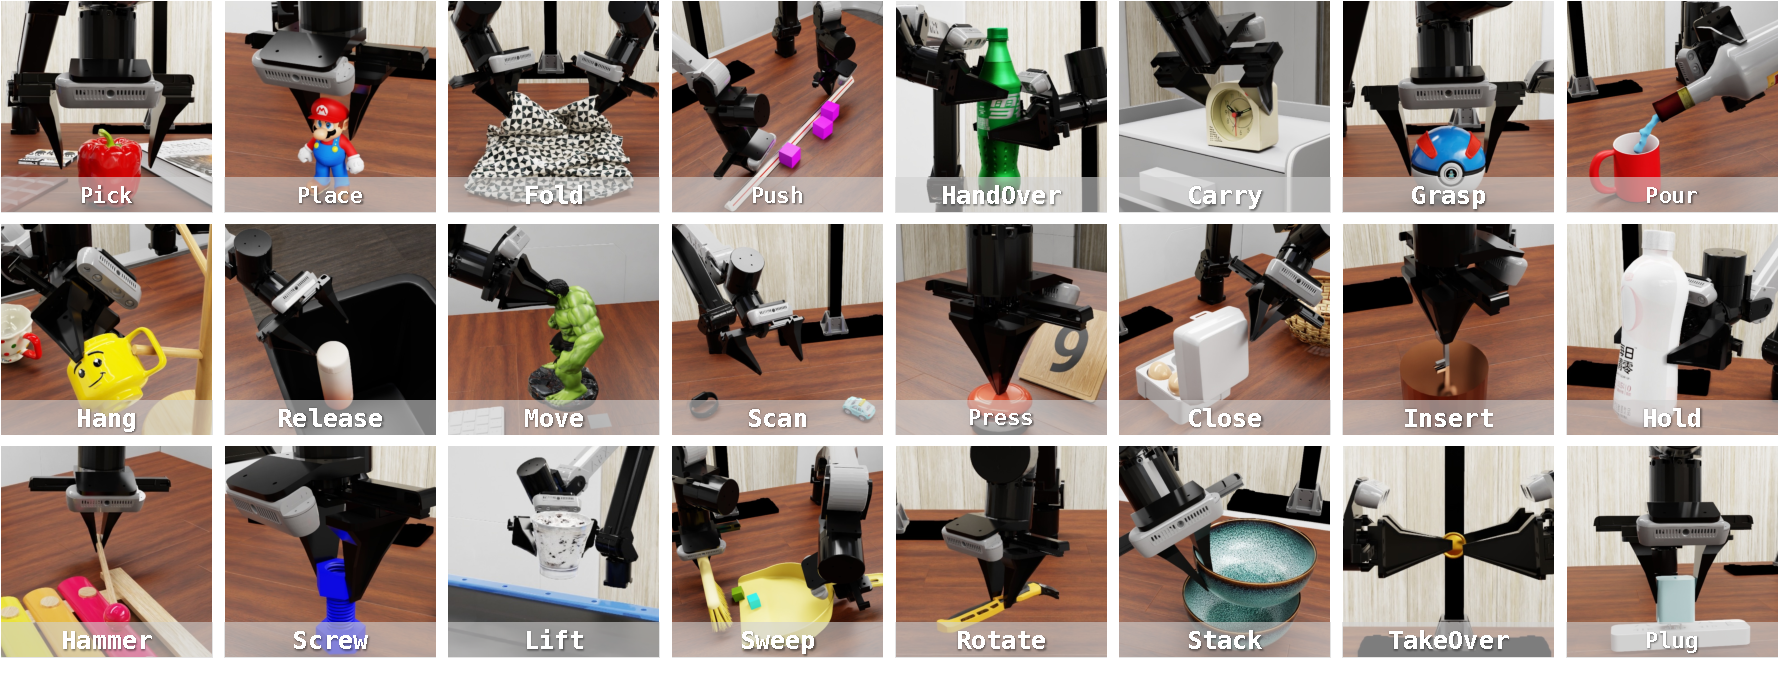
\includegraphics[width=1.0\textwidth]{assets/Figure/diverse_skills.pdf}
\caption{\textbf{Skill Diversity in RoboDojo.}
Representative simulation tasks cover 24 manipulation skills, including grasping, placing, pushing, pulling, stacking, insertion, opening, closing, folding, alignment, tool use, and contact-sensitive operations. These tasks span diverse spatial configurations and bimanual coordination patterns, enabling skill-level diagnosis beyond repetitive pick-and-place behaviors.}
\label{fig:skill_diversity}
\end{figure}

\subsection{Real-World Benchmark}

To evaluate policy performance under physical deployment conditions, we construct the \textbf{\textcolor{Blue_1}{RoboDojo Real-World Benchmark}}. The benchmark consists of 18 real-world tasks across three commonly used collaborative bimanual robot platforms: ARX X5, Piper, and Piper X. This multi-embodiment design evaluates whether policies can maintain reliable performance across different robot kinematics, workspaces, camera placements, and data distributions, rather than being specialized to a single platform.

Unlike simulation tasks, which support rapid feedback and capability-oriented diagnosis, the real-world benchmark exposes policies to deployment challenges that are difficult to fully capture in simulation, including contact-rich interactions, perception noise, actuation errors, workspace constraints, and temporal variations. As described in Section~\ref{sec:real_world_hardware}, we open-source the hardware setup and evaluation specifications of \textbf{RoboDojo-RealEval} to support reproducible deployment. RoboDojo-RealEval standardizes the hardware configuration, workspace layout, lighting condition, scene reset procedure, evaluation protocol, and deployment interface, enabling policies to be tested under consistent physical conditions. We further provide cloud-based remote evaluation, allowing users to submit policies and evaluate them under shared physical test configurations. Detailed task information is provided in Appendix~\ref{appendix:real_benchmark_tasks_details} and the \href{https://robodojo-benchmark.com/doc}{project documentation}.


\begin{figure}[t]
\centering
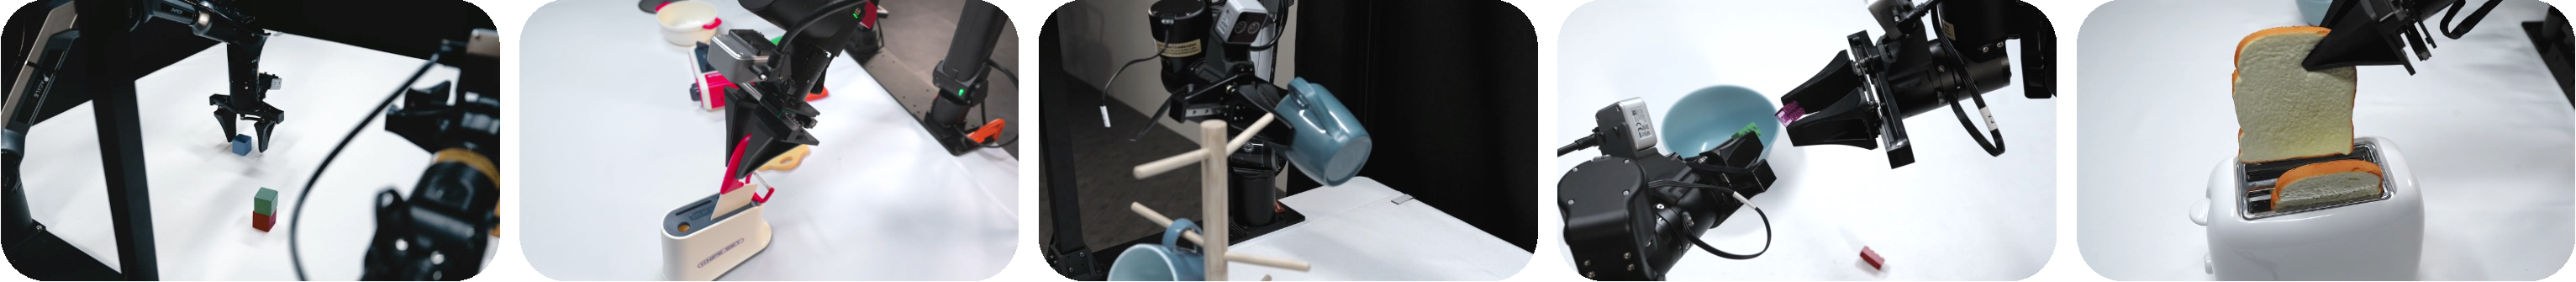
\includegraphics[width=1.0\textwidth]{assets/Figure/real_highlight.pdf}
\caption{\textbf{Real-World Task Highlights.} Representative key frames of challenging real-world manipulation tasks across different robot embodiments.}
\label{fig:real_highlight}
\end{figure}

\subsubsection{Task Design}

We design 6 tasks for each embodiment, resulting in 18 real-world tasks in total. Since real-world evaluation is constrained by hardware cost, execution time, human reset effort, and safety considerations, the benchmark is designed as a compact yet challenging physical test suite rather than an exhaustive enumeration of all capability dimensions. The selected tasks cover representative requirements, including long-horizon execution, precise manipulation, memory, and generalization.

Importantly, we do not construct one-to-one aligned task pairs between simulation and the real world. The real-world benchmark is not intended to measure direct sim-to-real transfer on matched tasks. Instead, it serves as a complementary evaluation setting for testing whether policies can handle physical deployment challenges beyond simulation success. The tasks involve contact-rich interactions, fine-grained spatial alignment, multi-object manipulation, partial observability, and embodiment-specific motion constraints, making evaluation sensitive to perception errors, actuation noise, accumulated trajectory drift, and unstable contact dynamics.

By evaluating policies across ARX X5, Piper, and Piper X under a shared protocol, RoboDojo assesses whether current generalist manipulation policies can operate reliably across diverse real-world deployment conditions. Detailed task specifications are provided in Appendix~\ref{appendix:real_benchmark_tasks_details}.

\subsubsection{Training Data Setting}

We collect real-world demonstrations using a homogeneous leader-follower teleoperation setup, where the leader arm has the same embodiment as the follower robot. This design aligns the teleoperation command space with the deployed robot embodiment, providing stable demonstrations for policy training. For each task, we collect 100 demonstrations from four operators to increase behavior diversity and reduce operator-specific bias. Across three embodiments and 18 tasks, the dataset contains 1,800 trajectories and 1,611,841 frames, corresponding to 17.91 hours of bimanual manipulation data recorded at 25~Hz.

Each demonstration includes robot states, language annotations, and synchronized RGB observations from one head camera and two wrist cameras. After collection, all trajectories are manually inspected for task completion, demonstration quality, and consistency with the RoboDojo-RealEval reset protocol. Detailed data modalities, filtering criteria, and embodiment-wise statistics are provided in Appendix~\ref{appendix:real_demo_statistics}.

\subsubsection{Evaluation Setting}

For real-world evaluation, we use the RoboDojo-RealEval platform introduced in Section~\ref{sec:real_world_hardware}. RoboDojo-RealEval supports both local deployment and remote cloud-based evaluation, where policies communicate with the real-robot client through the protocol described in Section~\ref{communication_protocol}. For each task, each policy is evaluated over 10 trials. Before each trial, a pre-collected evaluation layout is replayed to ensure consistent initial conditions across policies and sessions.

All trials are recorded and independently scored by three evaluators under a double-blind protocol. The scoring accounts for both final task success and intermediate sub-step completion, enabling fine-grained assessment of partial progress. The final score of each trial is computed as the average of the three evaluator scores. To improve transparency and fairness, we release evaluation videos and scores for leaderboard submissions, and provide an appeal mechanism for potential scoring errors. Additional details on motion planning, execution horizons, safety termination, and scoring protocols are provided in Appendix~\ref{appendix:real_evaluation_setting}.


\subsection{Evaluation Integrity and Anti-Gaming Protocols}

\begin{tcolorbox}[
colback=Blue_1!6,
colframe=Blue_1!65,
boxrule=0.6pt,
arc=2pt,
left=6pt,
right=6pt,
top=5pt,
bottom=5pt
]
\small
\textbf{\textcolor{Blue_1}{Leaderboard Governance.}}
The RoboDojo leaderboard is maintained by AI MMLab Club, a non-profit foundation dedicated to supporting open and community-driven AI research.
To ensure fairness, neutrality, and long-term credibility, RoboDojo evaluation will be jointly maintained and operated by global academic institutional partners.
No commercial company, including through sponsorship, funding, or operational participation, is involved in the official evaluation process.
As the benchmark evolves, the official evaluation and publication rules may be updated accordingly.
The latest leaderboard rules and submission protocol are available at
\href{http://RoboDojo-Benchmark.com/leaderboard}{http://RoboDojo-Benchmark.com/Leaderboard}.
\end{tcolorbox}

Although RoboDojo open-sources the simulation benchmark and the structural design of the real-world evaluation platform, official leaderboard publication requires a standardized verification protocol to ensure fairness, reproducibility, and community supervision. RoboDojo uses released public layouts as the primary leaderboard evaluation settings, allowing users to inspect task layouts, reproduce evaluations, and compare methods under a shared protocol. To reduce overfitting, hand-tuning, and leaderboard gaming on public layouts, submitted models are additionally evaluated on hidden verification layouts during official evaluation. These hidden layouts serve as an auxiliary consistency check rather than the primary leaderboard test set.

\begin{wrapfigure}{r}{0.35\linewidth}
    \vspace{-0.8em}
    \centering
    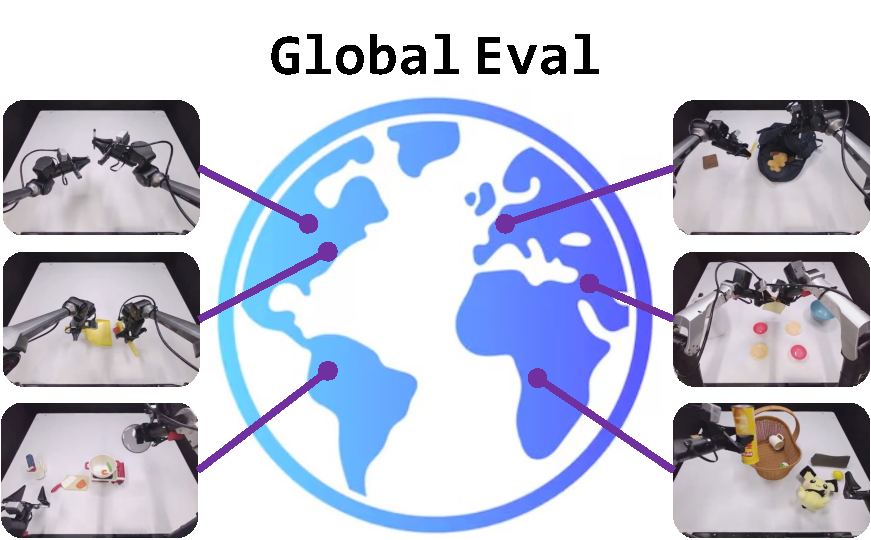
\includegraphics[width=0.95\linewidth]{assets/Figure/global_eval.pdf}
    \caption{\small RoboDojo official evaluation is jointly supported by global academic institutional partners, with no commercial participation.}
    \label{fig:global_eval}
    \vspace{-1.0em}
\end{wrapfigure}

RoboDojo supports remote evaluation without requiring participants to release checkpoints or source code during private development. Participants can run a remote policy server and communicate with the official RoboDojo evaluation client through the standardized deployment protocol. To publish results on the official verified leaderboard, each submission must satisfy the following requirements:
\textbf{(1)} policies are evaluated through the official RoboDojo online evaluation system;
\textbf{(2)} simulation results are reported over three random seeds with mean and standard deviation, and real-world results cover all three robot embodiments, including ARX X5, Piper, and Piper X;
\textbf{(3)} submitted models pass hidden-layout verification;
\textbf{(4)} the evaluated checkpoint, training and deployment code, configuration files, and reproducibility instructions are released through \textbf{XPolicyLab} at the leaderboard publication stage; and
\textbf{(5)} evaluation videos are released for community inspection.

Participants may still use RoboDojo for private evaluation and iteration without releasing code or checkpoints. However, results without the evaluated checkpoint, implementation, configuration files, and reproducibility instructions are reported separately and are not considered verified leaderboard entries. In this way, RoboDojo balances flexible remote development with a verified publication protocol that emphasizes reproducible policy performance rather than hand-tuned results on specific released layouts. Additional details of the verification and publication protocol are provided in Appendix~\ref{appendix:evaluation_integrity}.
